\documentclass[a4paper,11pt]{article}
\usepackage{amsmath,amssymb,amsthm, tikz,titlesec,hyperref,esint,braket, graphicx}

\usepackage[a4paper,margin=2cm]{geometry}
\linespread{1.3}
\newtheorem{claim}{Claim}[section]

\newcommand\name{Park Chanwoo}   % Name of the student
\newcommand\university{KAIST} % Name of the university
\newcommand\department{Physics} % Name of the department
\newcommand\studentid{20230297} % Student ID
\newcommand\s{\,\;}


\newenvironment{solution}[1]
  {\renewcommand\qedsymbol{$\square$}\begin{proof}[\textbf{Solution#1}]}
  {\end{proof}}
\newenvironment{note}
  {\renewcommand\qedsymbol{$\blacksquare$}\begin{proof}[\textnormal{\textbf{note}}]}
  {\end{proof}}

\title{KAIST\\2025 PH361 Solid State Physics I\\
Homework 3\bigskip}
\author{\textbf{\Large \name} \\
% University: \university\\
Department: \department\\
Student ID: \studentid}
\date{\today}

\begin{document}
\thispagestyle{empty}
\maketitle
\tableofcontents
\titleformat{\section}[frame]{\pagebreak}{\filright
\footnotesize  \enspace \textsf{KAIST --- PH361 Solid State Physics I 2025 Spring}\enspace}{6pt}{\Large\bfseries\filcenter}

\newcommand{\boltz}{k_{\mathrm{B}}}
\newcommand{\tr}{\operatorname{tr}}
\newcommand{\Li}{\operatorname{Li}}
\newcommand{\hc}{\text{h.c.}}
\newcommand{\cc}{\text{c.c.}}
\newcommand{\floor}{\operatorname{floor}}
\newcommand{\floor}{\operatorname{floor}}
\newcommand{\Re}{\operatorname{Re}}
\newcommand{\Im}{\operatorname{Im}}


\section{13.1 Reciprocal Lattice}

By definition, the FCC lattice with a conventional cube-edge $a$ is
\begin{equation}
    \mathcal L_{\mathrm{FCC}}(a_1, a_2, a_3)=\{n_1a_1\mathbf e_1+n_2a_2\mathbf e_2 + n_3a_3\mathbf e_3+\mathbf b:n_1, n_2, n_3\in\mathbb Z, \mathbf b\in\mathcal B\}
\end{equation}
Where
\begin{equation}
    \mathcal B=\{(0, 0, 0), (0, a_2/2, a_3/2), (a_1/2, 0, a_3/2), (a_1/2, a_2/2, 0)\}.
\end{equation}
Let's introducing the vectors,
\begin{align}
    \mathbf a_1&=(0, a_2/2, a_3/2),\\ 
    \mathbf a_2&=(a_1/2, 0, a_3/2),\\ 
    \mathbf a_3&=(a_1/2, a_2/2, 0)
\end{align}
Let
\begin{equation}
    \mathcal M=\{n_1\mathbf a_1+n_2\mathbf a_2 + n_3\mathbf a_3:n_1, n_2, n_3\in\mathbb Z\}.
\end{equation}
Since
\begin{align}
    a_1\mathbf e_1=\mathbf a_2 + \mathbf a_3 - \mathbf a_1, \\
    a_2\mathbf e_2=\mathbf a_3 + \mathbf a_1 - \mathbf a_2, \\
    a_3\mathbf e_3=\mathbf a_1 + \mathbf a_2 - \mathbf a_3,
\end{align}
every point in $\mathcal L_{\mathrm{FCC}}(a_1, a_2, a_3)$ can be represented by $n_1\mathbf a_1+n_2\mathbf a_2 + n_3\mathbf a_3$. Hence,
\begin{equation}
    \mathcal L_{\mathrm{FCC}}(a_1, a_2, a_3)\subseteq \mathcal M
\end{equation}
Also, 
\begin{equation}
    n_1\mathbf a_1+n_2\mathbf a_2 + n_3\mathbf a_3=\frac{n_2 + n_3}{2}a_1\mathbf e_1+\frac{n_3 + n_1}{2}a_2\mathbf e_2 + \frac{n_1 + n_2}{2}a_3\mathbf e_3
\end{equation}
and
\begin{equation}
    (n_2 + n_3) + (n_3 + n_1) + (n_1 + n_2) = 2(n_1+n_2+n_3)
\end{equation}
Since their sum is even, the integers $(n_2 + n_3), (n_3 + n_1), (n_1 + n_2)$ are all even or only two of them are odd. Therefore, there exist integers $m_1, m_2, m_3$ and $\mathbf b\in \{0, \mathbf a_1, \mathbf a_2, \mathbf a_3\}$, such that
\begin{equation}
    n_1\mathbf a_1+n_2\mathbf a_2 + n_3\mathbf a_3=a(m_1\mathbf e_1+m_2\mathbf e_2 + m_3\mathbf e_3) + \mathbf b.
\end{equation}
Thus, $\mathcal M\subseteq \mathcal L_{\mathrm{FCC}}(a_1, a_2, a_3)$ and they are equal
\begin{equation}
    \mathcal M = \mathcal L_{\mathrm{FCC}}(a_1, a_2, a_3)
\end{equation}
and $\mathbf a_1, \mathbf a_2, \mathbf a_3$ are a set of primitive lattice vectors of $\mathcal L_{\mathrm{FCC}}(a_1, a_2, a_3)$.

Let's consider the BCC lattice with a conventional cube-edge $a$:
\begin{equation}
    \mathcal L_{\mathrm{BCC}}(a_1, a_2, a_3) = \{n_1a_1\mathbf e_1+n_2a_2\mathbf e_2+n_3a_3\mathbf e_3 + \mathbf b:n_1, n_2, n_3\in \mathbb Z, \mathbf b\in\mathcal B\}
\end{equation}
Where
\begin{equation}
    \mathcal B=\{(0, 0, 0), (a_1/2, a_2/2, a_3/2)\}.
\end{equation}
Introduce the vectors,
\begin{align}
    \mathbf a_1&=(-a_1/2, a_2/2, a_3/2)\\
    \mathbf a_2&=(a_1/2, -a_2/2, a_3/2)\\
    \mathbf a_3&=(a_1/2, a_2/2, -a_3/2).
\end{align}
Then,
\begin{gather}
    a_1\mathbf e_1 = \mathbf a_2 + \mathbf a_3\\
    a_2\mathbf e_2 = \mathbf a_3 + \mathbf a_1\\
    a_3\mathbf e_3 = \mathbf a_1 + \mathbf a_2\\
    (a_1/2, a_2/2, a_3/2) = \mathbf a_1 + \mathbf a_2 + \mathbf a_3
\end{gather}
Hence,
\begin{equation}
    \mathcal L_{\mathrm{BCC}}(a_1, a_2, a_3)\subseteq \{n_1\mathbf a_1+n_2\mathbf a_2+n_3\mathbf a_3:n_1, n_2, n_3\in\mathbb Z\}.
\end{equation}
Conversely,
\begin{equation}
    n_1\mathbf a_1+n_2\mathbf a_2+n_3\mathbf a_3
    =\frac{n_2 + n_3 - n_1}{2}a\mathbf e_1+\frac{n_3 + n_1 - n_2}{2}a\mathbf e_2 + \frac{n_1 + n_2 - n_3}{2}a\mathbf e_3
\end{equation}
Let $n_1 + n_2 + n_3 = 2N + p$. where $N$ is an integer, and $p=0$ or $p=1$. Then,
\begin{align}
    n_1\mathbf a_1+n_2\mathbf a_2+n_3\mathbf a_3
    &=\frac{n_2 + n_3 - n_1}{2}a_1\mathbf e_1+\frac{n_3 + n_1 - n_2}{2}a_2\mathbf e_2 + \frac{n_1 + n_2 - n_3}{2}a_3\mathbf e_3\\
    &=(N - n_1)a_1\mathbf e_1+(N - n_2)a_2\mathbf e_2 + (N - n_3)a_3\mathbf e_3 + p(a_1/2, a_2/2, a_3/2).
\end{align}
Hence,
\begin{equation}
    \{n_1\mathbf a_1+n_2\mathbf a_2+n_3\mathbf a_3:n_1, n_2, n_3\in\mathbb Z\}\subseteq\mathcal L_{\mathrm{BCC}}(a_1, a_2, a_3).
\end{equation}
Therefore,
\begin{equation}
    \mathcal L_{\mathrm{BCC}}(a_1, a_2, a_3) = \{n_1\mathbf a_1+n_2\mathbf a_2+n_3\mathbf a_3:n_1, n_2, n_3\in\mathbb Z\}.
\end{equation}
and $\mathbf a_1, \mathbf a_2, \mathbf a_3$ is a set of primitive lattice vectors of $\mathcal L_{\mathrm{BCC}}(a_1, a_2, a_3)$.

Based on the above facts, let's find the reciprocal lattice of $\mathcal L_{\mathrm{FCC}}(a_1, a_2, a_3)$.

Let $\mathbf b_1, \mathbf b_2, \mathbf b_3$ be the vectors defined by
\begin{align}
    \mathbf b_1
    = \frac{2\pi (\mathbf a_2\times\mathbf a_3)}{\mathbf a_1\cdot(\mathbf a_2\times\mathbf a_3)}
    = \frac{4\pi}{a_1}(-1/2, 1/2, 1/2)\\
    \mathbf b_2
    = \frac{2\pi (\mathbf a_3\times\mathbf a_1)}{\mathbf a_2\cdot(\mathbf a_3\times\mathbf a_1)}
    = \frac{4\pi}{a_2}(1/2, -1/2, 1/2)\\
    \mathbf b_3
    = \frac{2\pi (\mathbf a_1\times\mathbf a_2)}{\mathbf a_3\cdot(\mathbf a_1\times\mathbf a_2)}
    = \frac{4\pi}{a_3}(1/2, 1/2, -1/2)
\end{align}
Where $\mathbf a_1, \mathbf a_2,\mathbf a_3$ is the set of primitive lattice vectors of $\mathcal L_{\mathrm{FCC}}(a_1, a_2, a_3)$ defined above.

Then $\mathbf a_i \cdot\mathbf b_j=2\pi \delta_{ij}$ . Because
\begin{equation}
    (n_1\mathbf a_1+n_2\mathbf a_2 + n_3\mathbf a_3) \cdot (m_1\mathbf b_1+m_2\mathbf b_2+m_3\mathbf b_3)=2\pi(n_1m_1+n_2m_2+n_3m_3)
\end{equation}
and
\begin{equation}
    e^{i(n_1\mathbf a_1+n_2\mathbf a_2 + n_3\mathbf a_3) \cdot (m_1\mathbf b_1+m_2\mathbf b_2+m_3\mathbf b_3)}=e^{2\pi i(n_1m_1+n_2m_2+n_3m_3)}=1.
\end{equation}
Therefore, the reciprocal lattice $\mathcal L_{\mathrm{FCC}}(a_1, a_2, a_3)$ of $\mathcal L_{\mathrm{FCC}}(a_1, a_2, a_3)$ is
\begin{equation}
    \mathcal L_{\mathrm{FCC}}^*(a_1, a_2, a_3)=\{n_1\mathbf b_1+n_2\mathbf b_2+n_3\mathbf b_3:n_1, n_2, n_3\in \mathbb Z\}=\mathcal L_{\mathrm{BCC}}(4\pi/a_1, 4\pi/a_2, 4\pi/a_3)
\end{equation}
Here $\mathcal L^*$ denotes the reciprocal of the lattice $\mathcal L$.

For an arbitrary lattice $\mathcal L$, suppose that $\mathcal M$ is the reciprocal lattice of the lattice $\mathcal L$, i.e., for every $\mathbf R\in\mathcal L$ and $\mathbf G\in\mathcal M$, $e^{i(\mathbf G\cdot\mathbf R)}=1$. This directly implies that for arbitrary $\mathbf G\in\mathcal M$, $e^{i(\mathbf R\cdot \mathbf G)}=e^{i(\mathbf G\cdot \mathbf R)}=1$ for every $\mathbf R\in\mathcal L$, which means that $\mathcal L$ is the reciprocal of $\mathcal M$. Therefore, $\mathcal L^*=\mathcal M$ if and only if $\mathcal M^*=\mathcal L$. 

Hence,
\begin{equation}
    \mathcal L_{\mathrm{BCC}}^*(4\pi/a_1, 4\pi/a_2, 4\pi/a_3)=\mathcal L_{\mathrm{FCC}}(a_1, a_2, a_3).
\end{equation}
by exchanging $a_1\leftrightarrow 4\pi/a_1$, $a_2\leftrightarrow 4\pi/a_2$, and $a_3\leftrightarrow 4\pi/a_3$,
\begin{equation}
    \mathcal L_{\mathrm{BCC}}^*(a_1, a_2, a_3)=\mathcal L_{\mathrm{FCC}}(4\pi/a_1, 4\pi/a_2, 4\pi/a_3).
\end{equation}

To sum up,

(a)
\begin{equation}
    \mathcal L_{\mathrm{BCC}}^*(a, a, a)=\mathcal L_{\mathrm{FCC}}(4\pi/a, 4\pi/a, 4\pi/a)
\end{equation}

(b)
\begin{equation}
    \mathcal L_{\mathrm{FCC}}^*(a, a, a)=\mathcal L_{\mathrm{BCC}}(4\pi/a, 4\pi/a, 4\pi/a).
\end{equation}

(c)\\
\begin{equation}
    \mathcal L_{\mathrm{FCC}}^*(a_1, a_2, a_3)=\mathcal L_{\mathrm{BCC}}(4\pi/a_1, 4\pi/a_2, 4\pi/a_3)
\end{equation}




\section{13.6 Brillouin Zones}

(a) For the cubic lattice $\mathcal L_{\text{cubic}}(a)=\{a\mathbf i:\mathbf i\in\mathbb Z^3\}$, the reciprocal lattice is $\mathcal L_{\text{cubic}}^*(a)=\{(2\pi/a)\mathbf i:\mathbf i\in\mathbb Z^3\}=\mathcal L_{\text{cubic}}(2\pi /a)$. The first Brillouin zone is $\mathrm{BZ}_1=[-\pi/a, \pi/a]^3$. 

For $\mathbf k=(k_x, k_y, k_z)\in\mathbb R^3$ and $\mathbf k'\in\mathrm{BZ}_1$,  they are equivalent if and only if there exists a reciprocal lattice vector $\mathbf G\in\mathcal L_{\text{cubic}}^*(a)$, such that $\mathbf k=\mathbf k'+ \mathbf G$. Let $f:\mathbb R\rightarrow [-\pi/a, \pi/a)$ such be defined by
\begin{equation}
    f(k)=x-\frac{2\pi}{a}\floor\left(\frac{a}{2\pi}k + \frac{1}{2}\right)
\end{equation}
Let $\mathbf k=(k_x, k_y, k_z)\in\mathbb R^3$, then $\mathbf k'=(f(k_x), f(k_y), f(k_z))\in\mathrm{BZ}_1$ , and they are equivalent since $\mathbf k=\mathbf k'+\mathbf G$ where $\mathbf G=(2\pi/a)(\floor((a/2\pi) k_x + 1/2), \floor((a/2\pi) k_y + 1/2), \floor((a/2\pi) k_z + 1/2))\in \mathcal L_{\text{cubic}}^*(a)$

(b) Let $\mathcal L_{\text{tri}}(a)=\{n_1\mathbf a_1+n_2\mathbf a_2:n_1, n_2\in\mathbb Z\}$, where $\mathbf a_1=a\mathbf e_1$ and $\mathbf a_2=\frac{a}{2}\mathbf e_1+\frac{\sqrt{3}a}{2}\mathbf e_2$. The reciprocal lattice is $\mathcal L_{\text{tri}}(a)=\{n_1\mathbf a_1^*+n_2\mathbf a_2^*:n_1, n_2\in\mathbb Z\}$, where $\mathbf a_1^*=\frac{2\pi}{a}\mathbf e_1-\frac{2\pi}{a\sqrt{3}}\mathbf e_2$ and $\mathbf a^*_2=\frac{4\pi}{a\sqrt{3}}\mathbf e_2$. Let $\mathbf a_3^*=\mathbf a_1^*+\mathbf a_2^*$. Then, the first Brillouin zone is the hexagon
\begin{align}
    \mathrm{BZ}_1
    &=\left\{\mathbf k\in\mathbb R^2:\frac{\mathbf a_{j}^*\cdot \mathbf k}{\|\mathbf a_j^*\|}\le\frac{\|\mathbf a_j^*\|}{2}, j=1,2,3\right\}\label{eqn:bz1}
\end{align}
Let's construct the mapping  $\mathbf k\mapsto \mathbf k'$. Define a function $f:\mathbb R\rightarrow [-1/2, 1/2)$ as
\begin{equation}
    f(x)=x-\floor\left(x+\frac{1}{2}\right)
\end{equation}
Then, the map 
\begin{equation}
    \mathbf k\mapsto \phi(\mathbf k)=f\left(\frac{\mathbf k\cdot\mathbf a_1}{2\pi}\right)\mathbf a_1^*+ f\left(\frac{\mathbf k\cdot\mathbf a_2}{2\pi}\right)\mathbf a_2^*
\end{equation}
maps to a Brillouin zone. But is not the first Brillouin zone. Hence, modify it a bit by the map $\rho$ so that $\rho(\phi(\mathbf k))\in\mathrm{BZ}_1$ which defined by
\begin{equation}
    \rho(\mathbf k)=\begin{cases}
        \mathbf k & \text{if $\mathbf k\in\mathrm{BZ}_1$}\\
        \mathbf k+\mathbf a_1^* &\text{if $k_x+k_y<0$ and $k_y>0$ and  $\mathbf k\notin\mathrm{BZ}_1$} \\
        \mathbf k-\mathbf a_1^* &\text{if $k_x+k_y>0$ and $k_y<0$ and  $\mathbf k\notin\mathrm{BZ}_1$}  \\
        \mathbf k+\mathbf a_2^* &\text{if $k_x+k_y<0$ and $k_y<0$ and  $\mathbf k\notin\mathrm{BZ}_1$}  \\
        \mathbf k-\mathbf a_2^* &\text{if $k_x+k_y>0$ and $k_y>0$ and  $\mathbf k\notin\mathrm{BZ}_1$}  \\
    \end{cases}
\end{equation}
The condition whether $\mathbf k\in \mathrm{BZ}_1$ or not can be easily tested by the condition shown in the Equation.~\ref{eqn:bz1}
. The composition $\rho\circ\phi$ maps an arbitrary $\mathbf k\in\mathbb R^2$ to its equivalent $\mathbf k'\in\mathrm{BZ}_1$.






\section{14.4 Neutron Scattering}

Since a hydrogen atom has only one electron, the response to electromagnetic waves is much less than other atoms, including sodium. Hence, the signal-to-noise ratio is not high enough for the hydrogen, X-ray scattering experiment is not a good method for positioning hydrogen atoms. For the neutron scattering, although hydrogen has a smaller cross section compared to the others,  

By the Fermi golden rule, the transition rate is
\begin{align}
    \Gamma_{\mathbf k'\leftarrow \mathbf k} 
    &= \frac{2\pi}{\hbar}|\bra{\mathbf k'}V\ket{\mathbf k}|^2\delta(E(\mathbf k')-E(\mathbf k)) \\
    &= \frac{\pi\hbar}{m}|\bra{\mathbf k'}V\ket{\mathbf k}|^2\delta(\|\mathbf k'\|^2-\|\mathbf k\|^2)
\end{align}
Using the box normalization,
\begin{align}
    \Gamma_{\mathbf k'\leftarrow \mathbf k} 
    &= \frac{\pi\hbar}{m}\left(\frac{1}{L^3}\int d\mathbf x\, e^{i(\mathbf k-\mathbf k')\cdot\mathbf x} V(\mathbf x)\right)^2\delta(\|\mathbf k'\|^2-\|\mathbf k\|^2) \\
    &= \frac{\pi\hbar}{m}\left(\frac{1}{L^3}\sum_{\mathbf R}\int_{\text{unit cell}} d\mathbf x\, e^{i(\mathbf k-\mathbf k')\cdot(\mathbf x+\mathbf R)} V(\mathbf x+\mathbf R)\right)^2\delta(\|\mathbf k'\|^2-\|\mathbf k\|^2) \\
    &= \frac{\pi\hbar}{m}\left(\frac{1}{L^3} \sum_{\mathbf R}e^{i(\mathbf k-\mathbf k')\cdot\mathbf R}\int_{\text{unit cell}} d\mathbf x\, e^{i(\mathbf k-\mathbf k')\cdot\mathbf x} V(\mathbf x)\right)^2\delta(\|\mathbf k'\|^2-\|\mathbf k\|^2)
\end{align}
Where $\frac{1}{L^3} \sum e^{i(\mathbf k-\mathbf k')\cdot\mathbf R}$ is the zero unless the $\mathbf k-\mathbf k'$ is a reciprocal lattice vector, which is the Laue condition. And the integral, the second term, is the structure factor $S(\mathbf G)=\int_{\text{unit cell}} d\mathbf x\, e^{i\mathbf G\cdot\mathbf x}V(\mathbf x)$. Whatever unit cell we take, the above formula holds. Hence, take a conventional unit cell for convenience.

Assume the potential is constructed by the two types of delta potentials: 
\begin{equation}
    V(\mathbf x)=f_{\mathrm{Na}}\sum_{\mathbf x'\in\mathcal B_{\mathrm{Na}}}\delta(\mathbf x-\mathbf x')+f_{\mathrm{H}}\sum_{\mathbf x'\in\mathcal B_{\mathrm{H}}}\delta(\mathbf x-\mathbf x')
\end{equation}
Then the structure factor is
\begin{align}
    S(\mathbf G)
    &=\int_{\text{unit cell}}d\mathbf x e^{i\mathbf G\cdot\mathbf x}V(\mathbf x) \\
    &=\int_{\text{unit cell}}d\mathbf x e^{i\mathbf G\cdot\mathbf x}\left[f_{\mathrm{Na}}\sum_{\mathbf x'\in\mathcal B_{\mathrm{Na}}}\delta(\mathbf x-\mathbf x')+f_{\mathrm{H}}\sum_{\mathbf x'\in\mathcal B_{\mathrm{H}}}\delta(\mathbf x-\mathbf x')\right]\\
    &=f_{\mathrm{Na}}\sum_{\mathbf x\in\mathcal B_{\mathrm{Na}}}e^{i\mathbf G\cdot\mathbf x}+f_{\mathrm{H}}\sum_{\mathbf x\in\mathcal B_{\mathrm{H}}}e^{i\mathbf G\cdot\mathbf x} \\
    &=(f_{\mathrm{Na}} + f_{\mathrm{H}}e^{i\mathbf G\cdot \mathbf y})\sum_{\mathbf x\in\mathcal B_{\mathrm{FCC}}}e^{i\mathbf G\cdot\mathbf x}
\end{align}

(i) for the sodium chloride structure, ($\mathbf y=[1/2, 1/2, 1/2]$):
\begin{equation}
    S_{hkl}=(f_{\mathrm{Na}} + f_{\mathrm{H}}e^{\pi i(h+k+l)})(1+e^{i\pi(h+k)}+e^{i\pi(k+l)}+e^{i\pi(l+h)})\\
\end{equation}
\begin{gather}
    S_{111}=4(f_{\mathrm{Na}} - f_{\mathrm{H}})\\
    S_{200}=4(f_{\mathrm{Na}} + f_{\mathrm{H}})\\
    \frac{8|S_{111}|^2}{6|S_{200}|^2} \approx\frac{8}{6}\left|\frac{0.374 + 0.363}{0.374 - 0.363}\right|^2\approx 5.985\times 10^3
\end{gather}
Since $\Gamma\propto (\text{multiplicity})|S|^2$, the calculated structure factor is consistent with the experimental result.


(ii) for the zinc blend structure, ($\mathbf y=[1/4, 1/4, 1/4]$):
\begin{equation}
    S_{hkl}=(f_{\mathrm{Na}} + f_{\mathrm{H}}e^{\pi i(h+k+l)/2})(1+e^{i\pi(h+k)}+e^{i\pi(k+l)}+e^{i\pi(l+h)})\\
\end{equation}
\begin{gather}
    S_{111}=4(f_{\mathrm{Na}} -i f_{\mathrm{H}})\\
    S_{200}=4(f_{\mathrm{Na}} - f_{\mathrm{H}})\\
    \frac{8|S_{111}|^2}{6|S_{200}|^2} \approx\frac{8}{6}\frac{0.374^2 + 0.363^2}{|0.374 + 0.363|^2}\approx 0.667
\end{gather}
Hence, the peak indexed as (200) must be higher. Based on the experimental result, the sample is not the $\mathrm{ZnS}$ structure.  

(b)
To filter a certain momentum state, we can use a velocity selector shown in the Figure.~\ref{fig:velocity-selector}.  Using the angular velocity that corresponds to the velocity that we want, we can filter the desired velocity from a non-monochromatic neutron source.
\begin{figure}
    \centering
    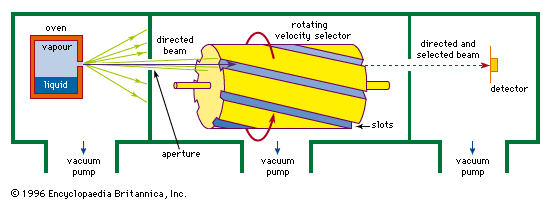
\includegraphics[width=0.5\linewidth]{HW3/velocity-selector.png}
    \caption{Velocity selector}
    \label{fig:velocity-selector}
\end{figure}


The key difference between X-ray scattering and neutron scattering is what it couples to. X-ray photons couple with electrons through electromagnetic interaction, while neutrons couple with nuclei through the nuclear force. Therefore, light elements such as hydrogen have fewer electrons, making them difficult to experiment with using X-rays while neutron scattering is effective for hydrogen atoms. Moreover, since neutrons interact directly with atomic nuclei, a mixture of different isotopes will give different results.

Since the relation between the energy and the momentum of a X-ray photon coupled with the speed of light, which is the very large constant, $E=pc$, it is hard to couple with a phonon which has the dispersion relation $E=\hbar\omega(k)=2\omega_0|\sin(ka/2)|$, because it is hard to conserve both the momentum and the energy. However, since the relation between the momentum and the kinetic energy of the neutron is $T=\frac{p^2}{2m}$, it is much easier to couple with phonons.


\section{14.9 Form Factors}

(a)
Start from the definition of the structure factor:
\begin{align}
    S(\mathbf G)
    &=\int_{\text{unit cell}} d\mathbf x\, e^{i\mathbf G\cdot\mathbf x}V(\mathbf x) \\
    &=\sum_{\alpha}\sum_{\mathbf R}\int_{\text{unit cell}} d\mathbf x\, e^{i\mathbf G\cdot\mathbf x}V_\alpha(\mathbf x - \mathbf R-\mathbf y_\alpha) \\
    &=\sum_{\alpha}\sum_{\mathbf R}\int_{\text{unit cell}} d\mathbf x\, e^{i\mathbf G\cdot\mathbf x}e^{-i\mathbf G\cdot\mathbf R}V_\alpha(\mathbf x - \mathbf R-\mathbf y_\alpha) \\
    &=\sum_{\alpha}\sum_{\mathbf R}\int_{\text{unit cell}} d\mathbf x\, e^{i\mathbf G\cdot(\mathbf x-\mathbf R)}V_\alpha(\mathbf x - \mathbf R-\mathbf y_\alpha) \\
    &=\sum_{\alpha}\int_{\mathbb R^3} d\mathbf x\, e^{i\mathbf G\cdot\mathbf x}V_\alpha(\mathbf x-\mathbf y_\alpha) \\
    &=\sum_{\alpha}\int_{\mathbb R^3-\mathbf y_\alpha} d(\mathbf x+\mathbf y_\alpha)\, e^{i\mathbf G\cdot(\mathbf x+\mathbf y_\alpha)}V_\alpha(\mathbf x) \\
    &=\sum_{\alpha}e^{i\mathbf G\cdot\mathbf y_\alpha}\int_{\mathbb R^3} d\mathbf x\, e^{i\mathbf G\cdot\mathbf x}V_\alpha(\mathbf x) 
\end{align}
by replacing the notation of the index $\alpha\rightarrow j$, and the positions of the atoms in a unit cell $\mathbf y_\alpha\rightarrow \mathbf x_j$, 
\begin{equation}
    S(\mathbf G)=\sum_{j}e^{i\mathbf G\cdot\mathbf x_j}\int_{\mathbb R^3} d\mathbf x\, e^{i\mathbf G\cdot\mathbf x}V_j(\mathbf x) 
\end{equation}
Hence, the form factor is
\begin{equation}
    f_j(\mathbf G)=\int_{\mathbb R^3} d\mathbf x\, e^{i\mathbf G\cdot\mathbf x}V_j(\mathbf x) 
\end{equation}
(b) 
\begin{align}
    f_j(\mathbf G)
    &=\int_{|\mathbf x| \le r_0^{(j)}}d\mathbf x\, e^{i\mathbf G\cdot\mathbf x}V_0^{(j)}\\
    &=V_0^{(j)}\int_{0}^{2\pi}d\phi\int_{0}^{r_0^{(j)}}r^2\,dr\int_{-1}^{1} \,d(\cos\theta)\, e^{i\|\mathbf G\|r\cos\theta}\\
    &=2\pi V_0^{(j)}\int_{0}^{r_0^{(j)}}r^2\,dr\frac{e^{i\|\mathbf G\|r}-e^{-i\|\mathbf G\|r}}{i\|\mathbf G\|r}\\
    &=2\pi V_0^{(j)}\frac{2}{\|\mathbf G\|}\int_{0}^{r_0^{(j)}}r\sin(\|\mathbf G\| r)\,dr\\
    &=2\pi V_0^{(j)}\frac{2}{\|\mathbf G\|}\int_{0}^{r_0^{(j)}}r\sin(\|\mathbf G\| r)\,dr\\
    &=4\pi  V_0^{(j)}\frac{\sin(\|\mathbf G\| r_0^{(j)})-\|\mathbf G\| r_0^{(j)}\cos(\|\mathbf G\| r_0^{(j)})}{\|\mathbf G\|^3}
\end{align}
The polar angle $\theta$ is chosen by the angle between $\mathbf G$ and $\mathbf x$. Let $x=\|\mathbf G\|r_0^{(j)}$
 and set $\frac{4}{3}\pi {r_0^{(j)}}^3 V_0^{(j)}=Z_{j}$ , which means $(\text{volume})\times(\text{energy})$,
\begin{equation}
    f_j(\mathbf G) = 3Z_j\frac{\sin x-x\cos x}{x^3}
\end{equation}

(c) X-ray fills the charge density $e|\psi|^2$ as a potential. Hence, let $V(\mathbf r)=C|\psi(\mathbf r)|^2$. The wavefunction of $1s$ orbital is
\begin{equation}
    \psi_{1s}(r)=\frac{1}{\sqrt{\pi}a_0^{3/2}}e^{-r/a_0}
\end{equation}
Where $a_0$ is the Bohr radius. hence the effective potential can be written by:
\begin{equation}
    V(r)=V_0e^{-2r/a_0}
\end{equation}
The form factor is
\begin{align}
    f_j(\mathbf G) 
    &= \int d\mathbf x\, e^{i\mathbf G\cdot\mathbf x}V(\|\mathbf x\|) \\
    &=V_0\int_0^{2\pi} d\phi\int_0^\infty r^2\, dr\int_{-1}^{1} d(\cos\theta) e^{i\|\mathbf G\|r\cos\theta}e^{-2r/a_0}\\
    &=\frac{4\pi V_0}{\|\mathbf G\|}\int_0^\infty r\sin(\|\mathbf G\|r) e^{-2r/a_0}\, dr\\
    &= \frac{16\pi V_0 a_0^3}{(4 + a_0^2\|\mathbf G\|^2)^2}
\end{align}
Hence, the form factor is proportional to $\frac{1}{(4 + a_0^2\|\mathbf G\|^2)^2}$




\end{document}
